% \documentclass{beamer}
\documentclass[hyperref={unicode}]{beamer}

\usepackage{amsmath}
\usepackage{datetime2}
\usepackage[numbers]{natbib}
\usepackage{graphicx}

\DTMnewdatestyle{mydateformat}{%
  \renewcommand{\DTMdisplaydate}[4]{%
    \number##1\ % year
    \DTMenglishmonthname{##2}\ % Month
    \number##3% day
  }%
  \renewcommand{\DTMDisplaydate}{\DTMdisplaydate}%
}
\DTMsetdatestyle{mydateformat}

\bibliographystyle{amsalpha}

\usetheme{Darmstadt}
\beamertemplatenavigationsymbolsempty

\title{Persistent Homology}
\subtitle{Computations and Applications}
\author{Stephen Ermshar}
\institute{Walla Walla University}
\date{\DTMDisplaydate{2020}{3}{13}{}}


\title{Persistent Homology}
\subtitle{Computations and Applications}
\author{Stephen Ermshar}
\institute{Walla Walla University}
\date{\DTMDisplaydate{2020}{3}{13}{}}

\begin{document}




\begin{frame}
    \titlepage
\end{frame}

\begin{frame}{Outline}
	\tableofcontents
\end{frame}

\section[Motivation]{Motivation}
\begin{frame}
	\textbf{Goal:} Given a collection of points in \(n\)-dimensional space, we want to reveal qualitative properties of an underlying shape that the points may have been sampled from.

	\begin{figure}
		\input{tikz-annulus-point-cloud-l23k29.tex}
		\caption{Motivation Example}
	\end{figure}
\end{frame}

\section[Homology]{Homology}
\subsection{\v{C}ech and Rips Complexes}
\begin{frame}
	\begin{block}{\v{C}ech Complex}
		\begin{align*}
			\textrm{\v{C}ech}(r) := \{ \sigma \subseteq P | \bigcap_{x\in \sigma} B_x(r) \neq \emptyset \}
		\end{align*}
		\cite{wagner}
	\end{block}
	\begin{figure}
		\input{tikz-example-cech-nl21k3j4.tex}
		\caption{A \v{C}ech Complex built from a point cloud.}
	\end{figure}
\end{frame}

% \begin{frame}
% 	\begin{block}{Rips Complex}
% 		\begin{align*}
% 			\textrm{Rips}(r) := \{ \sigma \subseteq P
% 				| \max_{a,b \in \sigma} d(a,b) < 2r \}
% 		\end{align*}
% 		\cite{wagner}
% 	\end{block}
% 	\begin{figure}
% 		\tikzset{
pattern size/.store in=\mcSize,
pattern size = 5pt,
pattern thickness/.store in=\mcThickness,
pattern thickness = 0.3pt,
pattern radius/.store in=\mcRadius,
pattern radius = 1pt}
\makeatletter
\pgfutil@ifundefined{pgf@pattern@name@_iy1rqtf17}{
\pgfdeclarepatternformonly[\mcThickness,\mcSize]{_iy1rqtf17}
{\pgfqpoint{0pt}{0pt}}
{\pgfpoint{\mcSize+\mcThickness}{\mcSize+\mcThickness}}
{\pgfpoint{\mcSize}{\mcSize}}
{
\pgfsetcolor{\tikz@pattern@color}
\pgfsetlinewidth{\mcThickness}
\pgfpathmoveto{\pgfqpoint{0pt}{0pt}}
\pgfpathlineto{\pgfpoint{\mcSize+\mcThickness}{\mcSize+\mcThickness}}
\pgfusepath{stroke}
}}
\makeatother
\tikzset{every picture/.style={line width=0.75pt}} %set default line width to 0.75pt

\begin{tikzpicture}[x=0.75pt,y=0.75pt,yscale=-1,xscale=1]
%uncomment if require: \path (0,95); %set diagram left start at 0, and has height of 95

\draw [shift={(163,23.5)}, rotate = 99.21] [color={rgb, 255:red, 165; green, 232; blue, 255}  ][fill={rgb, 255:red, 165; green, 232; blue, 255 }  ][line width=0]      (0, 0) circle [x radius= 20, y radius= 20]   ;
\draw [shift={(135,40)}, rotate = 349.29] [color={rgb, 255:red, 165; green, 232; blue, 255}  ][fill={rgb, 255:red, 165; green, 232; blue, 255 }  ][line width=0]      (0, 0) circle [x radius= 20, y radius= 20]   ;
\draw [shift={(13,61)}, rotate = 312.63] [color={rgb, 255:red, 165; green, 232; blue, 255}  ][fill={rgb, 255:red, 165; green, 232; blue, 255 }  ][line width=0]      (0, 0) circle [x radius= 20, y radius= 20]   ;
\draw [shift={(56,17)}, rotate = 0] [color={rgb, 255:red, 165; green, 232; blue, 255}  ][fill={rgb, 255:red, 165; green, 232; blue, 255 }  ][line width=0]      (0, 0) circle [x radius= 20, y radius= 20]   ;
\draw [shift={(69,54)}, rotate = 329.74] [color={rgb, 255:red, 165; green, 232; blue, 255}  ][fill={rgb, 255:red, 165; green, 232; blue, 255 }  ][line width=0]      (0, 0) circle [x radius= 20, y radius= 20]   ;
\draw [shift={(95,25)}, rotate = 353.99] [color={rgb, 255:red, 165; green, 232; blue, 255}  ][fill={rgb, 255:red, 165; green, 232; blue, 255 }  ][line width=0]      (0, 0) circle [x radius= 20, y radius= 20]   ;
\draw [shift={(95,25)}, rotate = 69.78] [color={rgb, 255:red, 165; green, 232; blue, 255}  ][fill={rgb, 255:red, 165; green, 232; blue, 255 }  ][line width=0]      (0, 0) circle [x radius= 20, y radius= 20]   ;
\draw [shift={(135,40)}, rotate = 314.34] [color={rgb, 255:red, 165; green, 232; blue, 255}  ][fill={rgb, 255:red, 165; green, 232; blue, 255 }  ][line width=0]      (0, 0) circle [x radius= 20, y radius= 20]   ;
\draw [shift={(157,60.5)}, rotate = 31.29] [color={rgb, 255:red, 165; green, 232; blue, 255}  ][fill={rgb, 255:red, 165; green, 232; blue, 255 }  ][line width=0]      (0, 0) circle [x radius= 20, y radius= 20]   ;
\draw [shift={(157,60.5)}, rotate = 349.29] [color={rgb, 255:red, 165; green, 232; blue, 255}  ][fill={rgb, 255:red, 165; green, 232; blue, 255 }  ][line width=0]      (0, 0) circle [x radius= 20, y radius= 20]   ;
\draw [shift={(157,60.5)}, rotate = 99.21] [color={rgb, 255:red, 165; green, 232; blue, 255}  ][fill={rgb, 255:red, 165; green, 232; blue, 255 }  ][line width=0]      (0, 0) circle [x radius= 20, y radius= 20]   ;
\draw [shift={(56,17)}, rotate = 312.63] [color={rgb, 255:red, 165; green, 232; blue, 255}  ][fill={rgb, 255:red, 165; green, 232; blue, 255 }  ][line width=0]      (0, 0) circle [x radius= 20, y radius= 20]   ;
\draw [shift={(95,25)}, rotate = 31.29] [color={rgb, 255:red, 165; green, 232; blue, 255}  ][fill={rgb, 255:red, 165; green, 232; blue, 255 }  ][line width=0]      (0, 0) circle [x radius= 20, y radius= 20]   ;
\draw [shift={(95,25)}, rotate = 0] [color={rgb, 255:red, 165; green, 232; blue, 255}  ][fill={rgb, 255:red, 165; green, 232; blue, 255 }  ][line width=0]      (0, 0) circle [x radius= 20, y radius= 20]   ;
\draw [shift={(69,54)}, rotate = 36.87] [color={rgb, 255:red, 165; green, 232; blue, 255}  ][fill={rgb, 255:red, 165; green, 232; blue, 255 }  ][line width=0]      (0, 0) circle [x radius= 20, y radius= 20]   ;
\draw [shift={(56,17)}, rotate = 36.87] [color={rgb, 255:red, 165; green, 232; blue, 255}  ][fill={rgb, 255:red, 165; green, 232; blue, 255 }  ][line width=0]      (0, 0) circle [x radius= 20, y radius= 20]   ;
\draw [shift={(95,25)}, rotate = 329.74] [color={rgb, 255:red, 165; green, 232; blue, 255}  ][fill={rgb, 255:red, 165; green, 232; blue, 255 }  ][line width=0]      (0, 0) circle [x radius= 20, y radius= 20]   ;
\draw [shift={(163,23.5)}, rotate = 353.99] [color={rgb, 255:red, 165; green, 232; blue, 255}  ][fill={rgb, 255:red, 165; green, 232; blue, 255 }  ][line width=0]      (0, 0) circle [x radius= 20, y radius= 20]   ;
\draw [shift={(135,40)}, rotate = 69.78] [color={rgb, 255:red, 165; green, 232; blue, 255}  ][fill={rgb, 255:red, 165; green, 232; blue, 255 }  ][line width=0]      (0, 0) circle [x radius= 20, y radius= 20]   ;
\draw [shift={(163,23.5)}, rotate = 314.34] [color={rgb, 255:red, 165; green, 232; blue, 255}  ][fill={rgb, 255:red, 165; green, 232; blue, 255 }  ][line width=0]      (0, 0) circle [x radius= 20, y radius= 20]   ;
\draw [shift={(255, 50)}, rotate = 314.34] [color={rgb, 255:red, 165; green, 232; blue, 255}  ][fill={rgb, 255:red, 165; green, 232; blue, 255 }  ][line width=0]      (0, 0) circle [x radius= 20, y radius= 20]   ;

%Straight Lines [id:da20686486428426965] (1-2)
% \draw    (13,61) -- (56,17) ;
\draw [shift={(56,17)}, rotate = 312.63] [color={rgb, 255:red, 0; green, 0; blue, 0 }  ][fill={rgb, 255:red, 0; green, 0; blue, 0 }  ][line width=0.75]      (0, 0) circle [x radius= 3.35, y radius= 3.35]   ;
\draw [shift={(13,61)}, rotate = 312.63] [color={rgb, 255:red, 0; green, 0; blue, 0 }  ][fill={rgb, 255:red, 0; green, 0; blue, 0 }  ][line width=0.75]      (0, 0) circle [x radius= 3.35, y radius= 3.35]   ;
%Straight Lines [id:da9899744043809231] (2-4)
\draw    (56,17) -- (95,25) ;
% \draw [shift={(95,25)}, rotate = 0] [color={rgb, 255:red, 0; green, 0; blue, 0 }  ][fill={rgb, 255:red, 0; green, 0; blue, 0 }  ][line width=0.75]      (0, 0) circle [x radius= 3.35, y radius= 3.35]   ;
% \draw [shift={(56,17)}, rotate = 0] [color={rgb, 255:red, 0; green, 0; blue, 0 }  ][fill={rgb, 255:red, 0; green, 0; blue, 0 }  ][line width=0.75]      (0, 0) circle [x radius= 3.35, y radius= 3.35]   ;
%Straight Lines [id:da4483952202454973] (2-3)
\draw    (56,17) -- (69,54) ;
\draw [shift={(69,54)}, rotate = 36.87] [color={rgb, 255:red, 0; green, 0; blue, 0 }  ][fill={rgb, 255:red, 0; green, 0; blue, 0 }  ][line width=0.75]      (0, 0) circle [x radius= 3.35, y radius= 3.35]   ;
\draw [shift={(56,17)}, rotate = 36.87] [color={rgb, 255:red, 0; green, 0; blue, 0 }  ][fill={rgb, 255:red, 0; green, 0; blue, 0 }  ][line width=0.75]      (0, 0) circle [x radius= 3.35, y radius= 3.35]   ;
%Straight Lines [id:da013663715151336797](3-4)
\draw    (69,54) -- (95,25) ;
\draw [shift={(95,25)}, rotate = 329.74] [color={rgb, 255:red, 0; green, 0; blue, 0 }  ][fill={rgb, 255:red, 0; green, 0; blue, 0 }  ][line width=0.75]      (0, 0) circle [x radius= 3.35, y radius= 3.35]   ;
\draw [shift={(69,54)}, rotate = 329.74] [color={rgb, 255:red, 0; green, 0; blue, 0 }  ][fill={rgb, 255:red, 0; green, 0; blue, 0 }  ][line width=0.75]      (0, 0) circle [x radius= 3.35, y radius= 3.35]   ;
%Straight Lines [id:da6445202628566384](4-7)
% \draw    (95,25) -- (163,23.5) ;
\draw [shift={(163,23.5)}, rotate = 353.99] [color={rgb, 255:red, 0; green, 0; blue, 0 }  ][fill={rgb, 255:red, 0; green, 0; blue, 0 }  ][line width=0.75]      (0, 0) circle [x radius= 3.35, y radius= 3.35]   ;
\draw [shift={(95,25)}, rotate = 353.99] [color={rgb, 255:red, 0; green, 0; blue, 0 }  ][fill={rgb, 255:red, 0; green, 0; blue, 0 }  ][line width=0.75]      (0, 0) circle [x radius= 3.35, y radius= 3.35]   ;
%Straight Lines [id:da3743946516627876] (4-5)
% \draw    (95,25) -- (135,40) ;
\draw [shift={(135,40)}, rotate = 69.78] [color={rgb, 255:red, 0; green, 0; blue, 0 }  ][fill={rgb, 255:red, 0; green, 0; blue, 0 }  ][line width=0.75]      (0, 0) circle [x radius= 3.35, y radius= 3.35]   ;
\draw [shift={(95,25)}, rotate = 69.78] [color={rgb, 255:red, 0; green, 0; blue, 0 }  ][fill={rgb, 255:red, 0; green, 0; blue, 0 }  ][line width=0.75]      (0, 0) circle [x radius= 3.35, y radius= 3.35]   ;
%Straight Lines [id:da2401873796980163] (5-7)
\draw    (135,40) -- (163,23.5) ;
\draw [shift={(163,23.5)}, rotate = 314.34] [color={rgb, 255:red, 0; green, 0; blue, 0 }  ][fill={rgb, 255:red, 0; green, 0; blue, 0 }  ][line width=0.75]      (0, 0) circle [x radius= 3.35, y radius= 3.35]   ;
\draw [shift={(135,40)}, rotate = 314.34] [color={rgb, 255:red, 0; green, 0; blue, 0 }  ][fill={rgb, 255:red, 0; green, 0; blue, 0 }  ][line width=0.75]      (0, 0) circle [x radius= 3.35, y radius= 3.35]   ;
%Straight Lines [id:da08347218855288774] (4-6)
% \draw    (95,25) -- (157,60.5) ;
\draw [shift={(157,60.5)}, rotate = 31.29] [color={rgb, 255:red, 0; green, 0; blue, 0 }  ][fill={rgb, 255:red, 0; green, 0; blue, 0 }  ][line width=0.75]      (0, 0) circle [x radius= 3.35, y radius= 3.35]   ;
\draw [shift={(95,25)}, rotate = 31.29] [color={rgb, 255:red, 0; green, 0; blue, 0 }  ][fill={rgb, 255:red, 0; green, 0; blue, 0 }  ][line width=0.75]      (0, 0) circle [x radius= 3.35, y radius= 3.35]   ;
%Straight Lines [id:da34695654406224863]
\draw    (135,40) -- (157,60.5) ;
\draw [shift={(157,60.5)}, rotate = 349.29] [color={rgb, 255:red, 0; green, 0; blue, 0 }  ][fill={rgb, 255:red, 0; green, 0; blue, 0 }  ][line width=0.75]      (0, 0) circle [x radius= 3.35, y radius= 3.35]   ;
\draw [shift={(135,40)}, rotate = 349.29] [color={rgb, 255:red, 0; green, 0; blue, 0 }  ][fill={rgb, 255:red, 0; green, 0; blue, 0 }  ][line width=0.75]      (0, 0) circle [x radius= 3.35, y radius= 3.35]   ;
%Straight Lines [id:da5097015872445443]
\draw    (163,23.5) -- (157,60.5) ;
\draw [shift={(157,60.5)}, rotate = 99.21] [color={rgb, 255:red, 0; green, 0; blue, 0 }  ][fill={rgb, 255:red, 0; green, 0; blue, 0 }  ][line width=0.75]      (0, 0) circle [x radius= 3.35, y radius= 3.35]   ;
\draw [shift={(163,23.5)}, rotate = 99.21] [color={rgb, 255:red, 0; green, 0; blue, 0 }  ][fill={rgb, 255:red, 0; green, 0; blue, 0 }  ][line width=0.75]      (0, 0) circle [x radius= 3.35, y radius= 3.35]   ;

\draw [pattern=_iy1rqtf17,pattern size=6pt,pattern thickness=0.75pt,pattern radius=0pt, pattern color={rgb, 255:red, 0; green, 0; blue, 0}] (135,40) -- (163,23.5) -- (157,60.5) -- cycle ;


\draw [pattern=_iy1rqtf17,pattern size=6pt,pattern thickness=0.75pt,pattern radius=0pt, pattern color={rgb, 255:red, 0; green, 0; blue, 0}] (56,17) -- (69,54) -- (95,25) -- cycle ;

% Text Node
\draw (27.5,66.5) node    {$1$};
% Text Node
\draw (65,10) node    {$2$};
% Text Node
\draw (80,58.5) node    {$3$};
% Text Node
\draw (105,16) node    {$4$};
% Text Node
\draw (130,50) node    {$5$};
% Text Node
\draw (172,62) node    {$6$};
% Text Node
\draw (176,13.5) node    {$7$};
% Text Node
\draw[fill={rgb, 255:red, 0; green, 0; blue, 0 }] (255, 50) circle [x radius= 3.35, y radius= 3.35]    (260,40) node    {$8$};



\end{tikzpicture}

% 		\caption{A Rips Complex built from a point cloud.}
% 	\end{figure}
% \end{frame}

\subsection{Simplicial Homology}
\begin{frame}
	\begin{definition}
		An oriented \textbf{n-Simplex} will be represented as an tuple of \(n+1\) vertices.
	\end{definition}
	\begin{figure}
		\input{tikz-basic-simplices-1m42sd.tex}
		\caption{Examples of basic simplices.}
	\end{figure}
\end{frame}

\begin{frame}
	\begin{definition}
		A \textbf{Simplicial Complex} is a finite collection of finite sets such that every subset of every element in the collection is also an element in the collection. \cite{wagner}
	\end{definition}
	\begin{figure}
		\tikzset{every picture/.style={line width=0.75pt}} %set default line width to 0.75pt

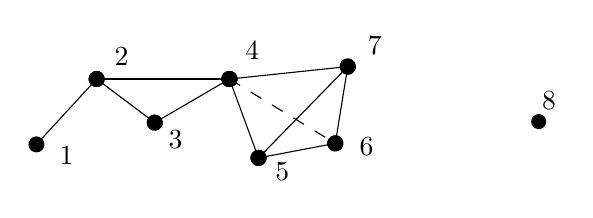
\begin{tikzpicture}[x=0.75pt,y=0.75pt,yscale=-1,xscale=1]
%uncomment if require: \path (0,95); %set diagram left start at 0, and has height of 95

%Straight Lines [id:da20686486428426965]
\draw    (13,61) -- (42,29.5) ;
\draw [shift={(42,29.5)}, rotate = 312.63] [color={rgb, 255:red, 0; green, 0; blue, 0 }  ][fill={rgb, 255:red, 0; green, 0; blue, 0 }  ][line width=0.75]      (0, 0) circle [x radius= 3.35, y radius= 3.35]   ;
\draw [shift={(13,61)}, rotate = 312.63] [color={rgb, 255:red, 0; green, 0; blue, 0 }  ][fill={rgb, 255:red, 0; green, 0; blue, 0 }  ][line width=0.75]      (0, 0) circle [x radius= 3.35, y radius= 3.35]   ;
%Straight Lines [id:da9899744043809231]
\draw    (42,29.5) -- (106,29.5) ;
\draw [shift={(106,29.5)}, rotate = 0] [color={rgb, 255:red, 0; green, 0; blue, 0 }  ][fill={rgb, 255:red, 0; green, 0; blue, 0 }  ][line width=0.75]      (0, 0) circle [x radius= 3.35, y radius= 3.35]   ;
\draw [shift={(42,29.5)}, rotate = 0] [color={rgb, 255:red, 0; green, 0; blue, 0 }  ][fill={rgb, 255:red, 0; green, 0; blue, 0 }  ][line width=0.75]      (0, 0) circle [x radius= 3.35, y radius= 3.35]   ;
%Straight Lines [id:da4483952202454973]
\draw    (42,29.5) -- (70,50.5) ;
\draw [shift={(70,50.5)}, rotate = 36.87] [color={rgb, 255:red, 0; green, 0; blue, 0 }  ][fill={rgb, 255:red, 0; green, 0; blue, 0 }  ][line width=0.75]      (0, 0) circle [x radius= 3.35, y radius= 3.35]   ;
\draw [shift={(42,29.5)}, rotate = 36.87] [color={rgb, 255:red, 0; green, 0; blue, 0 }  ][fill={rgb, 255:red, 0; green, 0; blue, 0 }  ][line width=0.75]      (0, 0) circle [x radius= 3.35, y radius= 3.35]   ;
%Straight Lines [id:da013663715151336797]
\draw    (70,50.5) -- (106,29.5) ;
\draw [shift={(106,29.5)}, rotate = 329.74] [color={rgb, 255:red, 0; green, 0; blue, 0 }  ][fill={rgb, 255:red, 0; green, 0; blue, 0 }  ][line width=0.75]      (0, 0) circle [x radius= 3.35, y radius= 3.35]   ;
\draw [shift={(70,50.5)}, rotate = 329.74] [color={rgb, 255:red, 0; green, 0; blue, 0 }  ][fill={rgb, 255:red, 0; green, 0; blue, 0 }  ][line width=0.75]      (0, 0) circle [x radius= 3.35, y radius= 3.35]   ;
%Straight Lines [id:da6445202628566384]
\draw    (106,29.5) -- (163,23.5) ;
\draw [shift={(163,23.5)}, rotate = 353.99] [color={rgb, 255:red, 0; green, 0; blue, 0 }  ][fill={rgb, 255:red, 0; green, 0; blue, 0 }  ][line width=0.75]      (0, 0) circle [x radius= 3.35, y radius= 3.35]   ;
\draw [shift={(106,29.5)}, rotate = 353.99] [color={rgb, 255:red, 0; green, 0; blue, 0 }  ][fill={rgb, 255:red, 0; green, 0; blue, 0 }  ][line width=0.75]      (0, 0) circle [x radius= 3.35, y radius= 3.35]   ;
%Straight Lines [id:da3743946516627876]
\draw    (106,29.5) -- (120,67.5) ;
\draw [shift={(120,67.5)}, rotate = 69.78] [color={rgb, 255:red, 0; green, 0; blue, 0 }  ][fill={rgb, 255:red, 0; green, 0; blue, 0 }  ][line width=0.75]      (0, 0) circle [x radius= 3.35, y radius= 3.35]   ;
\draw [shift={(106,29.5)}, rotate = 69.78] [color={rgb, 255:red, 0; green, 0; blue, 0 }  ][fill={rgb, 255:red, 0; green, 0; blue, 0 }  ][line width=0.75]      (0, 0) circle [x radius= 3.35, y radius= 3.35]   ;
%Straight Lines [id:da2401873796980163]
\draw    (120,67.5) -- (163,23.5) ;
\draw [shift={(163,23.5)}, rotate = 314.34] [color={rgb, 255:red, 0; green, 0; blue, 0 }  ][fill={rgb, 255:red, 0; green, 0; blue, 0 }  ][line width=0.75]      (0, 0) circle [x radius= 3.35, y radius= 3.35]   ;
\draw [shift={(120,67.5)}, rotate = 314.34] [color={rgb, 255:red, 0; green, 0; blue, 0 }  ][fill={rgb, 255:red, 0; green, 0; blue, 0 }  ][line width=0.75]      (0, 0) circle [x radius= 3.35, y radius= 3.35]   ;
%Straight Lines [id:da08347218855288774]
\draw  [dash pattern={on 4.5pt off 4.5pt}]  (106,29.5) -- (157,60.5) ;
\draw [shift={(157,60.5)}, rotate = 31.29] [color={rgb, 255:red, 0; green, 0; blue, 0 }  ][fill={rgb, 255:red, 0; green, 0; blue, 0 }  ][line width=0.75]      (0, 0) circle [x radius= 3.35, y radius= 3.35]   ;
\draw [shift={(106,29.5)}, rotate = 31.29] [color={rgb, 255:red, 0; green, 0; blue, 0 }  ][fill={rgb, 255:red, 0; green, 0; blue, 0 }  ][line width=0.75]      (0, 0) circle [x radius= 3.35, y radius= 3.35]   ;
%Straight Lines [id:da34695654406224863]
\draw    (120,67.5) -- (157,60.5) ;
\draw [shift={(157,60.5)}, rotate = 349.29] [color={rgb, 255:red, 0; green, 0; blue, 0 }  ][fill={rgb, 255:red, 0; green, 0; blue, 0 }  ][line width=0.75]      (0, 0) circle [x radius= 3.35, y radius= 3.35]   ;
\draw [shift={(120,67.5)}, rotate = 349.29] [color={rgb, 255:red, 0; green, 0; blue, 0 }  ][fill={rgb, 255:red, 0; green, 0; blue, 0 }  ][line width=0.75]      (0, 0) circle [x radius= 3.35, y radius= 3.35]   ;
%Straight Lines [id:da5097015872445443]
\draw    (163,23.5) -- (157,60.5) ;
\draw [shift={(157,60.5)}, rotate = 99.21] [color={rgb, 255:red, 0; green, 0; blue, 0 }  ][fill={rgb, 255:red, 0; green, 0; blue, 0 }  ][line width=0.75]      (0, 0) circle [x radius= 3.35, y radius= 3.35]   ;
\draw [shift={(163,23.5)}, rotate = 99.21] [color={rgb, 255:red, 0; green, 0; blue, 0 }  ][fill={rgb, 255:red, 0; green, 0; blue, 0 }  ][line width=0.75]      (0, 0) circle [x radius= 3.35, y radius= 3.35]   ;


% Text Node
\draw (27.5,66.5) node    {$1$};
% Text Node
\draw (54,18.5) node    {$2$};
% Text Node
\draw (80,58.5) node    {$3$};
% Text Node
\draw (117,16) node    {$4$};
% Text Node
\draw (131.5,74) node    {$5$};
% Text Node
\draw (172,62) node    {$6$};
% Text Node
\draw (176,13.5) node    {$7$};
% Text Node
\draw[fill={rgb, 255:red, 0; green, 0; blue, 0 }] (255, 50) circle [x radius= 3.35, y radius= 3.35]    (260,40) node    {$8$};



\end{tikzpicture}

		\caption{Example simplicial complex with two connected components, one hole, and one void.}
	\end{figure}
	\begin{align*}
		C = \{
			&(4,5,7), (5,6,7), (4,6,7), (4,5,6),\quad (1,2), (2,3),\\ &(3,4), (2,4), (4,5), (5,6),(6,7),(4,7),(4,6),(5,7),\\
			&(1), (2), (3), (4), (5), (6), (7), (8)
		\}
	\end{align*}
\end{frame}

\begin{frame}
	\begin{definition}
		The \textbf{Boundary Homomorphism} \(\partial_n : C_n \to C_{n-1}\) maps elements from the group of \(n\)-simplicies to elements in the group of \((n-1)\)-simplicies and is defined by
		\[
			\partial_n (v_0,\dots , v_{n}) = \sum_{i=0}^n (-1)^{i}
			(v_0,\dots, \widehat{v_i}, \dots, v_n)
		\]
		\cite{hatcher}
	\end{definition}
	\begin{align*}
		\partial_2 (4,5,7) = (5,7) - (4,7) + (4,5)
	\end{align*}
	\begin{align*}
		\partial_1 [(5,7) - (4,7) + (4,5)] = (7) - (5) - (7) + (4) + (5) - (4) = 0
	\end{align*}
\end{frame}

\begin{frame}
	\begin{definition}
		The \textbf{n-th Homology Group} is \(H_n = \bigslant{\Ker(\partial_n)}{\Ima(\partial_{n+1})}\)
		\cite{fraleigha}
	\end{definition}
\end{frame}

\subsection{Computations}
\begin{frame}
	\begin{figure}
		\input{tikz-homology-calc-example-lkj3h4.tex}
		\caption{A simple complex for calculating homology groups.}
	\end{figure}
	\begin{align*}
		&C_2 = \langle (1,2,3) \rangle \\
		&C_1 = \langle (1,2),(1,3),(2,3),(2,4),(3,4) \rangle \\
	\end{align*}
	\begin{align*}
		\Ima (\partial_2) = \langle (2,3) - (1,3) + (2,3) \rangle \simeq \Z
	\end{align*}
\end{frame}

\begin{frame}
	\begin{figure}
		\input{tikz-homology-calc-example-lkj3h4.tex}
		\caption{A simple complex for calculating homology groups.}
	\end{figure}
	\begin{align*}
		&C_2 = \langle (1,2,3) \rangle \\
		&C_1 = \langle (1,2),(1,3),(2,3),(2,4),(3,4) \rangle \\
	\end{align*}
	\begin{align*}
		\Ima (\partial_2) = \langle (2,3) - (1,3) + (2,3) \rangle \simeq \Z
	\end{align*}
\end{frame}





\section[Persistence]{Persistent Homology}
\subsection{Persistence Diagrams}
\begin{frame}
\end{frame}

\section{Applications}
\subsection{Visualization, Compression, and Data Segmentation}
\begin{frame}
\end{frame}

\section*{Bibliography}
\begin{frame}{Bibliography}
	\nocite{wagner}
	\nocite{hatcher}
	\nocite{fraleigha}
	% https://tex.stackexchange.com/a/22654
	\begingroup
	\renewcommand{\section}[2]{}%
	\bibliography{../math496-7-zotero.bib}
	\endgroup
\end{frame}




\end{document}
